\documentclass[letterpaper]{article}
\usepackage[T1]{fontenc}
\usepackage{textcomp}
\usepackage{mathptmx}
\usepackage[scaled=0.9]{helvet}
\usepackage{url}
\usepackage{graphicx}
\setcounter{secnumdepth}{-2}
\title{Google Affiliate Network Plugin User Manual}
\author{Robert Heller}
\date{\today}
\begin{document}

\maketitle

\tableofcontents

\section{Introduction}

I wrote this plugin to display ads from the Google Affiliate Network on
Deepwoods Software's WordPress powered website. This plugin uses a
database of ads to display.  The ads are displayed in rotation, using
the simple method of counting ad impressions and giving priority to the
advertisers with the least impressions and display ads with the least
impressions first that are expiring soonest.  As ads and advertisers
are displayed, their impression counts are incremented, which moves
them down the list\footnote{To the back of the list once the impression
counts reach equilibrium, when the impression counts are all the
same.}.  This means that all ads are displayed fairly, with preference
given to new ads and to ads which are expiring soonest\footnote{Expired
ads are not displayed and a daily cron job deletes them.}. After using
``in house'' for a while, I have made this plugin available to other
WordPress users who also using the Google Affiliate Network as a source
of advertising revenue.

\subsection{Sustainable Plugin Development - and Your Privacy}

Google Affiliate Network is a participant in the Sustainable Plugins
Sponsorship Network (SPSN) - \url{http://pluginsponsors.com/}. The SPSN
model offers modest sponsorships to plugin authors in return for a
small amount of screen real estate on plugin options pages. The SPSN
sponsor messages can be switched altogether: just visit the Config
page.

\textbf{IMPORTANT PRIVACY INFORMATION: NO INDIVIDUALLY IDENTIFIABLE
DETAILS OF ANY KIND, REGARDING EITHER YOU OR YOUR SITE}, will be
collected or shared as a result of displaying Sustainable Plugins
Sponsorship Network (SPSN) sponsor messages. Sponsors receive only
aggregate reports of impressions on a worldwide per-plugin basis, NOT
on impressions or on any other activity at any individual site which
happens to be using a plugin.

There is a configuration option to disable PluginSponsor messages, see
the section on configuring for details about this option.

\section{Installation}

Installation is just a matter of installing from the new plugin
page.  Once installed and activated, the plugin is ready to start
displaying affiliate ads.

\section{Configuring}

There are two configuration options: one for automatically deleting
expired ads and one to disable PluginSponsor messages.  The option to
automatically delete expired ads is on by default and the option to
disable PluginSponsor messages is off by default. While it is possible
to disable automatically deleting expired ads it is not recommended. If
PluginSponsor messages are turned off, a PayPal donate message is
displayed instead.

If you have upgraded from an older version of the plugin, the
configure page will display a button to upgrade the database to the new
version.

\section{Managing your ad database}

\begin{figure}[ht]
\begin{centering}
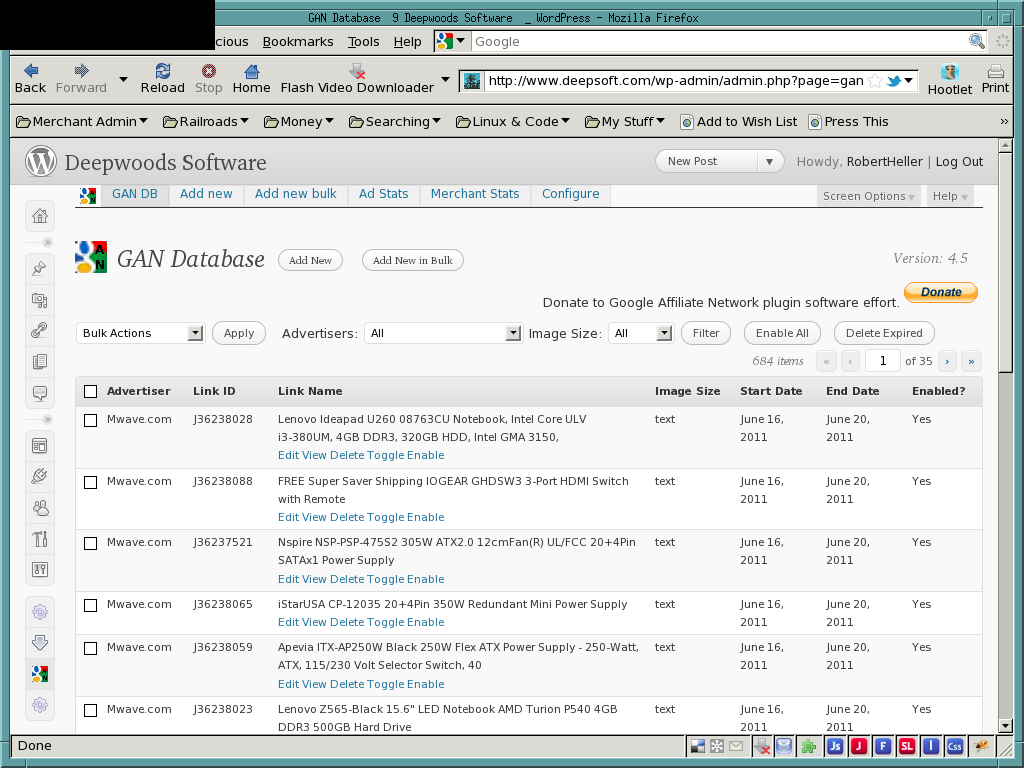
\includegraphics[width=3in]{gandatabase.png}
\caption{GAN Database Admin Page}
\label{fig:gandb}
\end{centering}
\end{figure}
Managing your ads is done from the main GAN database page, shown in
Figure~\ref{fig:gandb}. The advertiser, link id, link name, image size,
start date, end date, and enabled flag are displayed in this table. Ads
are sorted by increasing end date.  It is possible to filter the
displayed ad by advertiser and/or ad size.  There is a button to enable
all ads and to delete ads that have expired.  Ads can be deleted or
have their enable flag toggled in bulk.  Ads can be individually
edited, viewed, deleted or have their enable flags toggled.

\subsection{Inserting Ads}

In order to display ads, you need to have some ads in your database.
There are two ways to insert ads: manually, one by one or in bulk from
a TSV (Tab Separated Value) file. Manual insertion is done on the
\emph{Add new} admin page and bulk insertion is done on the
\emph{Add new bulk} admin page.

\subsubsection{Add new admin page (manual insertion)}

\begin{figure}[ht]
\begin{centering}
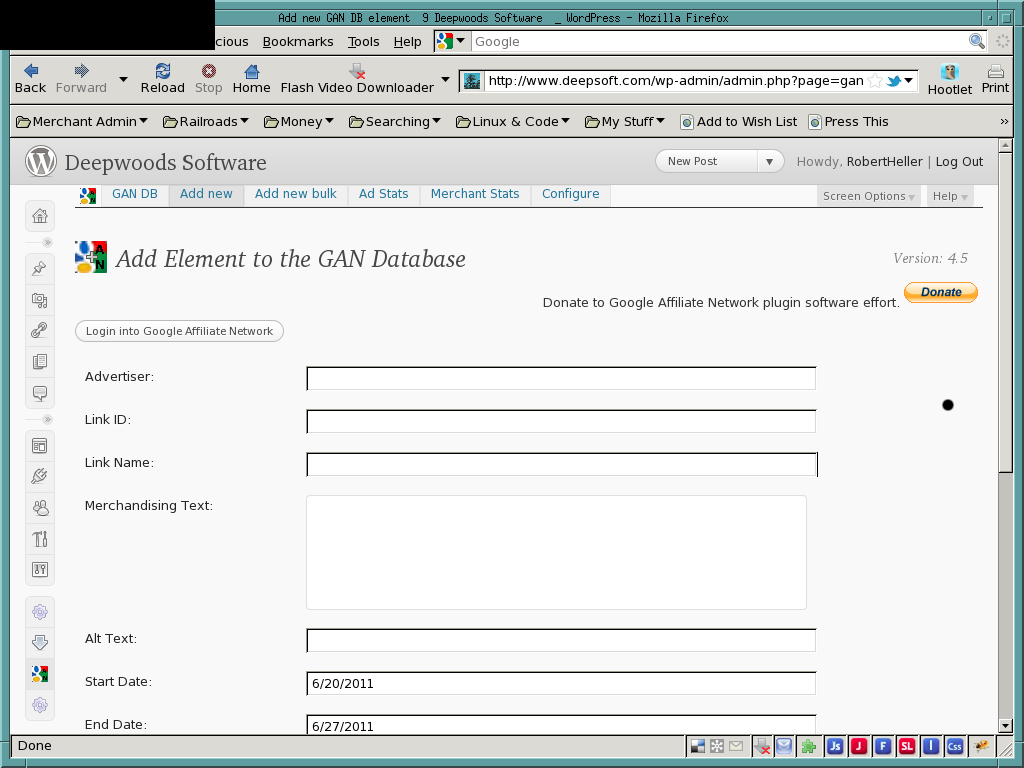
\includegraphics[width=3in]{ganmanualadd.png}
\caption{GAN Manual Add Page}
\label{fig:manualadd}
\end{centering}
\end{figure}
This page, shown in Figure~\ref{fig:manualadd}, has a form for adding
(and editing and viewing) a single ad. Generally, this page is not
usually used, see Section~\ref{sect:addbulk} for adding ads in bulk.
The fields\footnote{These fields correspond to the column headings used
in the files sent as part of your E-Mailed Link Subscriptions.}
include: 

\begin{description}
  \item[Advertiser:] This is the advertiser's name.
  \item[Link ID:] This is the (unique) Link Id code. This ID value is
supplied by Google and uniquely identifies the ad.  Link IDs must be
unique and are prefixed by an uppercase ``J''.
  \item[Link Name:] This is the name of the link.  It is used as the
anchor text for text ads.
  \item[Merchandising Text:] This is some ad copy for the
link and is displayed with the ad link.
  \item[Alt Text:] This is the alternative text for image
ads.
  \item[Start Date:] The is the starting date, in the format yyyy-mm-dd
or m/d/yyyy. 
  \item[End Date:] This is the ending date, in the format yyyy-mm-dd or
m/d/yyyy. For ads with no ending date use a date far into the future,
like 2037-12-31.
  \item[Clickserver Link:] This is the tracking URL for the ad. 
  \item[ImageURL:] This is the URL of the ad image for image ads. 
  \item[ImageHeight:] This is the height of the image (0 for text ads). 
  \item[ImageWidth:] This is the width of the image (0 for text ads). 
  \item[LinkURL:] This is the Link URL.  This is the URL of the actual
banner image.
  \item[PromoType:] This is the type of promotion.
  \item[MerchantID:] This is the (unique) merchant id.  This value is
supplied by Google and is prefixed by a uppercase ``K''.
  \item[enabled?] This indicates of the ad is enabled or
not. 
\end{description}

\subsubsection{Add new bulk admin page (bulk insertion)}
\label{sect:addbulk}

\begin{figure}[ht]
\begin{centering}
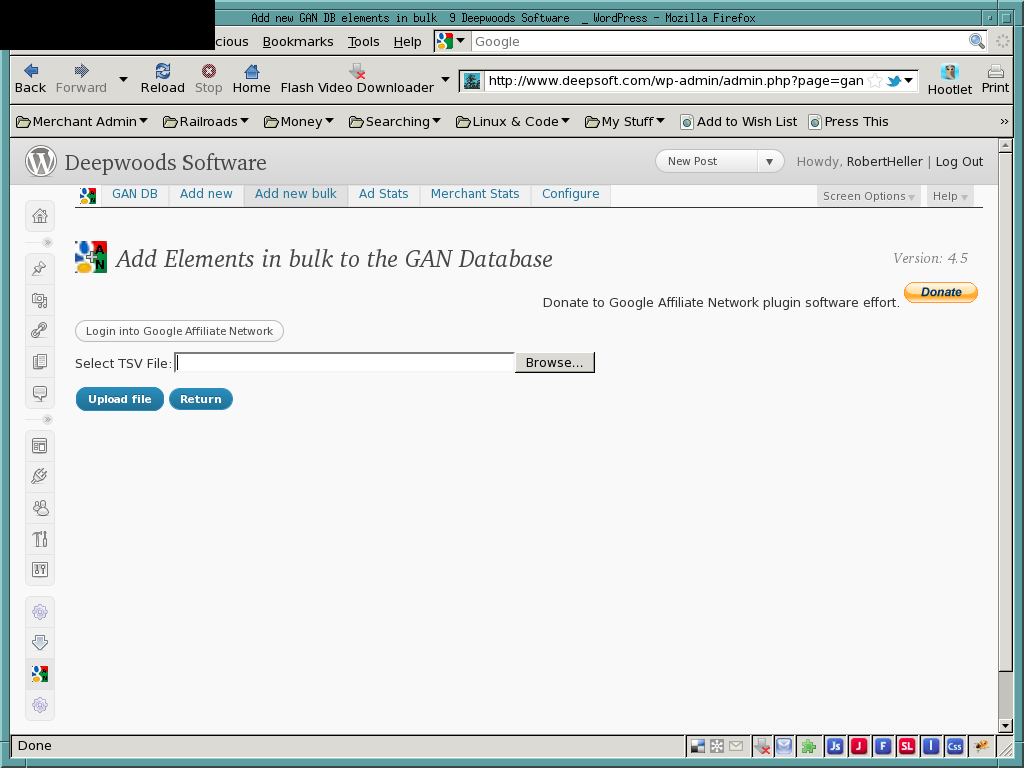
\includegraphics[width=3in]{bulkadd.png}
\caption{GAN Bulk Add Page}
\label{fig:bulkadd}
\end{centering}
\end{figure}
\begin{figure}[ht]
\begin{centering}
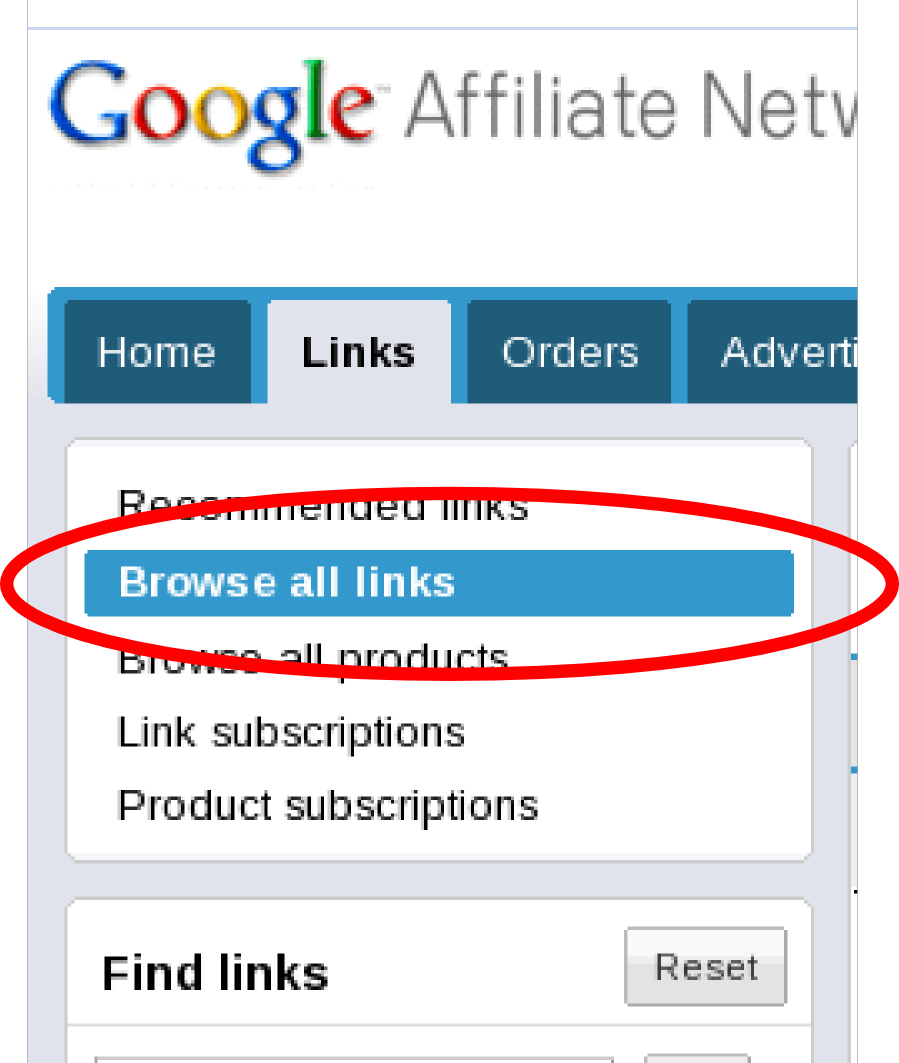
\includegraphics[width=2in]{ganLinksTab.png}
\caption{GAN Links Tab}
\label{fig:ganLinksTab}
\end{centering}
\end{figure}
\begin{figure}[ht]
\begin{centering}
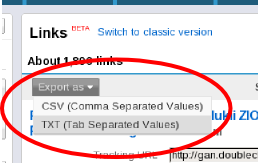
\includegraphics[width=2in]{ganExport.png}
\caption{GAN Export Links As}
\label{fig:ganExport}
\end{centering}
\end{figure}
This page, shown in Figure~\ref{fig:bulkadd}, uploads a TSV file of ads
previously downloaded from your Google Affiliate Network management
page. You get this file by visiting your Google Affiliate Network
management page and clicking the Links tab (see
figure~\ref{fig:ganLinksTab}). On this page you can select the sorts of
ads you would like by selecting one or more of your approved
advertisers and selecting the type of ads (text and/or banner), and
other criteria such as size, etc. It is then possible to export these
ads as a TSV file, using the Export As button and selecting ``Tab
Separated Values'' option (see figure~\ref{fig:ganExport}), which can
then be downloaded. This same file can in turn be uploaded to the GAN
plugin and the ads in this file will be added to your ad database.

\subsection{Editing Ads}

When displaying the data on the main admin page, links are provided
to edit, delete, or toggle the enabled flag for each ad. The ads are
displayed ordered by expiration date, with the soonest to expire
displayed first. It is possible to select only a single merchant's ads
to be displayed and/or a single size of ad or only text ads.

\subsection{Ad Subscriptions}

A Tcl script is included to process E-Mailed Ad Subscriptions and
insert them into the database.  This requires the ability to receive
E-Mail on the server running the database server and requires that Tcl
and the MySQLTcl package be installed as well as the use of procmail as
a mail delivery agent.

\section{Showing Ads}

There are two ways to show ads on your pages and/or posts.  You can
use one of the two widgets (GAN Image Widget or GAN Widget) or one of
the two shortcodes (GAN\_Text or GAN\_Image).  The widgets of course need
to go into a 'sidebar' that supports widgets.  The shortcodes can go
into any post or page.

\subsection{GAN Widget}

\begin{figure}[ht]
\begin{centering}
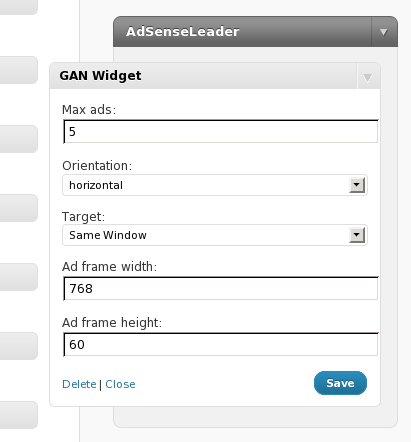
\includegraphics[width=2in]{ganwidget.png}
\caption{GAN Widget}
\label{fig:ganwidget}
\end{centering}
\end{figure}
This widget (see Figure~\ref{fig:ganwidget}) shows text ads in a
``sidebar'' that supports widgets.

The GAN Widget has five parameters:
\begin{description}
  \item[Max ads:] The maximum number of ads to display in this ad unit.
  \item[Orientation:] The orientation of the ads. Horizontal
means the ads are arranged side by side like one row of a table and
vertical means the ads are arranged in a vertical list. Typically the
horizontal orientation is suitable for a wide but short ad frame and the
vertical orientation is suitable for sky scrapper type ad unit.
  \item[Target:] The link target to use. Can be either Same 
Window or New Window or Tab.
  \item[Ad frame width:] The width of the ad frame. A value
of zero will cause the frame to use all of the available space.
  \item[Ad frame height:] The height of the ad frame.
\end{description}

\subsection{GAN Image Widget}

\begin{figure}[ht]
\begin{centering}
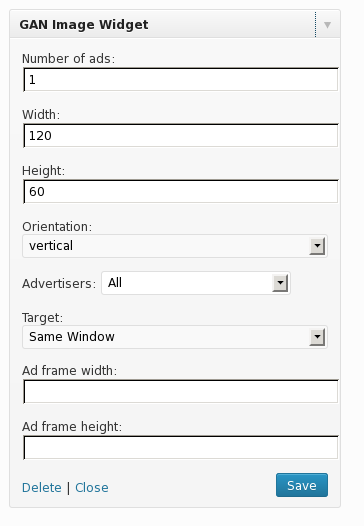
\includegraphics[width=2in]{ganimagewidget.png}
\caption{GAN Image Widget}
\label{fig:ganimagewidget}
\end{centering}
\end{figure}
This widget (see Figure~\ref{fig:ganimagewidget}) shows image (banner) 
ads in a ``sidebar'' that supports widgets.  Any given widget instance
(ad unit) can only show one size of banner ad.

The GAN Image Widget has seven parameters:
\begin{description}
  \item[Max ads:] The maximum number of ads to display in this ad unit.
  \item[Width:] The image width of the image ads.
  \item[Height:] The image height of the image ads.
  \item[Orientation:] The orientation of the ads. Horizontal
means the ads are arranged side by side like one row of a table and
vertical means the ads are arranged in a vertical list. Typically the
horizontal orientation is suitable for a wide but short ad frame and the
vertical orientation is suitable for sky scrapper type ad unit.
  \item[Target:] The link target to use. Can be either Same 
Window or New Window or Tab.
  \item[Ad frame width:] The width of the ad frame. A value
of zero will cause the frame to use all of the available space.
  \item[Ad frame height:] The height of the ad frame.
\end{description}

\subsection{GAN\_Text shortcode}

This shortcode inserts a text ad unit into a page or post.

The GAN\_Text shortcode has same five parameters as the GAN
Widget:
\begin{description}
  \item[maxads] An integer, with the default being 4.
The maximum number of ads to display in this ad unit.
  \item[orientation] The orientation of the ads, one of
``vertical'' (the default) or ``horizontal''. Horizontal means the ads are
arranged side by side like one row of a table and      vertical means
the ads are arranged in a vertical list. Typically the horizontal
orientation is suitable for a wide but short ad frame and the vertical
orientation is suitable for sky scrapper type ad unit.
  \item[target] The link target to use, one of ``same'' (the
default) or ``new''.
  \item[ifwidth] The width of the ad frame. A value
of zero will cause the frame to use all of the available space.
  \item[ifheight] The height of the ad frame.
\end{description}

Here is an example -- 5 text ads arranged horizontally in a 798x70 frame:
\begin{verbatim}
[GAN_Text maxads=5 orientation='horizontal' ifwidth=798 ifheight=70]
\end{verbatim}

\subsection{GAN\_Image shortcode}

This shortcode inserts an image (banner) ad unit into a page or post.
Like the GAN Image Widget, all of the ads displayed are of the same
size. 

The GAN\_Image shortcode has same seven parameters as the GAN Image
Widget:
\begin{description}
  \item[maxads] An integer, with the default being 4.
The maximum number of ads to display in this ad unit.
  \item[orientation] The orientation of the ads, one of
``vertical'' (the default) or ``horizontal''. Horizontal means the ads are
arranged side by side like one row of a table and      vertical means
the ads are arranged in a vertical list. Typically the horizontal
orientation is suitable for a wide but short ad frame and the vertical
orientation is suitable for sky scrapper type ad unit.
  \item[target] The link target to use, one of ``same'' (the
default) or ``new''.
  \item[width] The image width of the image ads. The
default is 120.
  \item[height] The image height of the image ads. The
default is 60.
  \item[ifwidth] The width of the ad frame. A value
of zero will cause the frame to use all of the available space.
  \item[ifheight] The height of the ad frame.
\end{description}

Here is an example -- 2 468x60 banners arranged vertically in a 468x126 frame:
\begin{verbatim}
[GAN_Image maxads=2 orientation='vertical' ifwidth=468 ifheight=126 width=468 height=60]
\end{verbatim}

\subsection{Using the ad unit insertion media button}


\begin{figure}[ht]
\begin{centering}
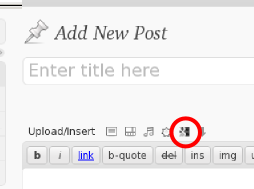
\includegraphics[width=2in]{ganmediabutton.png}
\caption{GAN Insert Ad Unit Media button}
\label{fig:ganmediabutton}
\end{centering}
\end{figure}
\begin{figure}[ht]
\begin{centering}
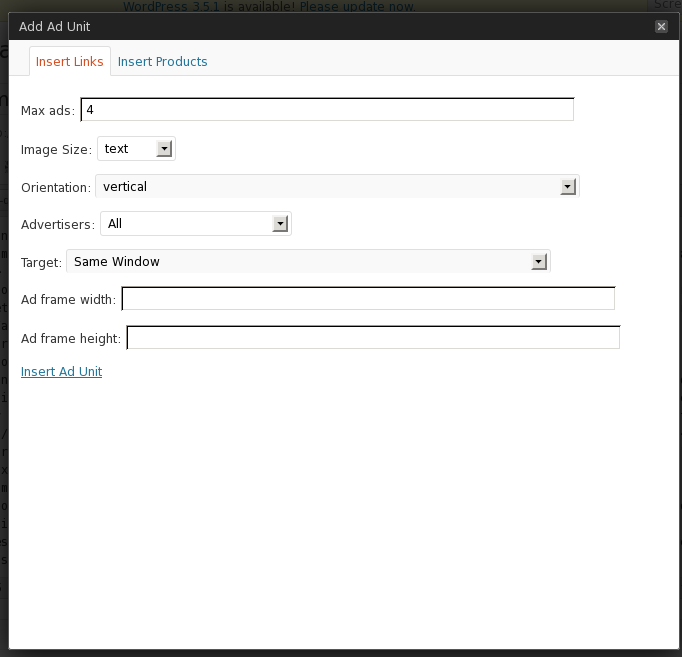
\includegraphics[width=3in]{ganinsertaddialog.png}
\caption{GAN Insert Ad Unit Dialog Box}
\label{fig:ganinsertaddialog}
\end{centering}
\end{figure}
As of version 4.3, a ``media button'', shown in
Figure~\ref{fig:ganmediabutton}, is available to aid in the insertion
of the ad unit short codes into pages and posts.  This button opens a
dialog window, shown in Figure~\ref{fig:ganinsertaddialog}, where the
parameters can be easily selected to create a short code that will
insert an ad unit into the current page or post. You can select the
maximumn number of ads to display in this ad unit, the size or type of
ad, the orientation of the ads within the ad unit and the size of the
ad frame. When you click on the insert ad button, the proper short code
is generated and inserted into your page or post.

\subsection{The ad rotation algorithmn}

The ad rotation algorithmn uses the impression count and the end date to
fairly display ads.  Impression counts are stored for each ad and each
merchant.  When an ad from a given merchant is displayed, that
merchant's impression count is incremented.  And when a given ad is
displayed, its impression count is incremented.  These counts are used
like this:

The ad display loop works like this:

First the merchant with the lowest impression count that has an ad of
the desired size is selected.  Then the ad from that merchant with the
lowest impression count, that also has the soonest end date is selected
(expired ads are not shown).  The HTML code for the ad is generated,
then the impression count for the ad and the merchant are incremented.
Then the process is repeated.  This means that every merchant gets a
shot and every ad of every merchant also gets a shot.

Some things to note:

If a merchant has a lot of ads, each of these ads will be displayed
fewer times than the ads of a merchant with a smaller number of ads. 
Each merchant will get the same number of total impressions and these
impressions will be shared across all of the merchant's ads.  Ads that
will expire sooner will get ``prefered'' exposure and will tend to get
more impressions, at least until they expire.  Newly added merchants and
ads will also get ``prefered'' exposure, since they will be starting
with a impression counts of zero.  But over time, these ``new''
merchants and ads will catch up with the older merchants and ads.  It is
possible to zero the impression counts of both merchants and ads and
this will ``level'' the playing field.

\section{Statistics}

Both ad and merchant statistics are available for display and download
as CSV files.  The statistics are ordered from fewest impressions to
most impressions. A summary of the statistics is also displayed on the
dashboard.  Ad statistics can be filtered by advertiser and/or by size.

In the statistics display is the option to zero all, a select group, or
individual ads or merchants. These impression counts are used by the ad
rotation algorithmn.

\end{document}



